\documentclass[10pt, a4paper]{extarticle}
\usepackage[T1]{fontenc}
\usepackage[english]{babel}
\usepackage[margin=1cm]{geometry}
\usepackage[utf8]{inputenc}
\usepackage{graphicx}
\usepackage{hyperref}
\usepackage{natbib}
\usepackage{microtype}
% List spacing
\usepackage{enumitem}
% Source Sans Pro font
\usepackage{sourcesanspro}
\renewcommand{\familydefault}{\sfdefault}
% Cambria font
%\usepackage{fontspec}
%\setmainfont[Ligatures=TeX]{Cambria}

% Headings format
\usepackage{titlesec}

\renewcommand{\bibsection}{\section*{Publications}}
\bibliographystyle{plainnat}
% Disable page number
\pagenumbering{gobble}


% Paragraph spacing
\usepackage{parskip}
% Headings

\titleformat*{\section}{\normalfont\large\bfseries}%\color{MidnightBlue}}

\titleformat*{\subsection}{\bfseries}%\color{MidnightBlue}}
% Title format
\makeatletter
\def\@maketitle{
\newpage
{\LARGE\textbf{{\@title}} \par}

Bologna, Italy | \href{mailto:kmfrick98@gmail.com}{\texttt{kmfrick98@gmail.com}}  | \url{https://kmfrick.tech}
%\hfill\smash{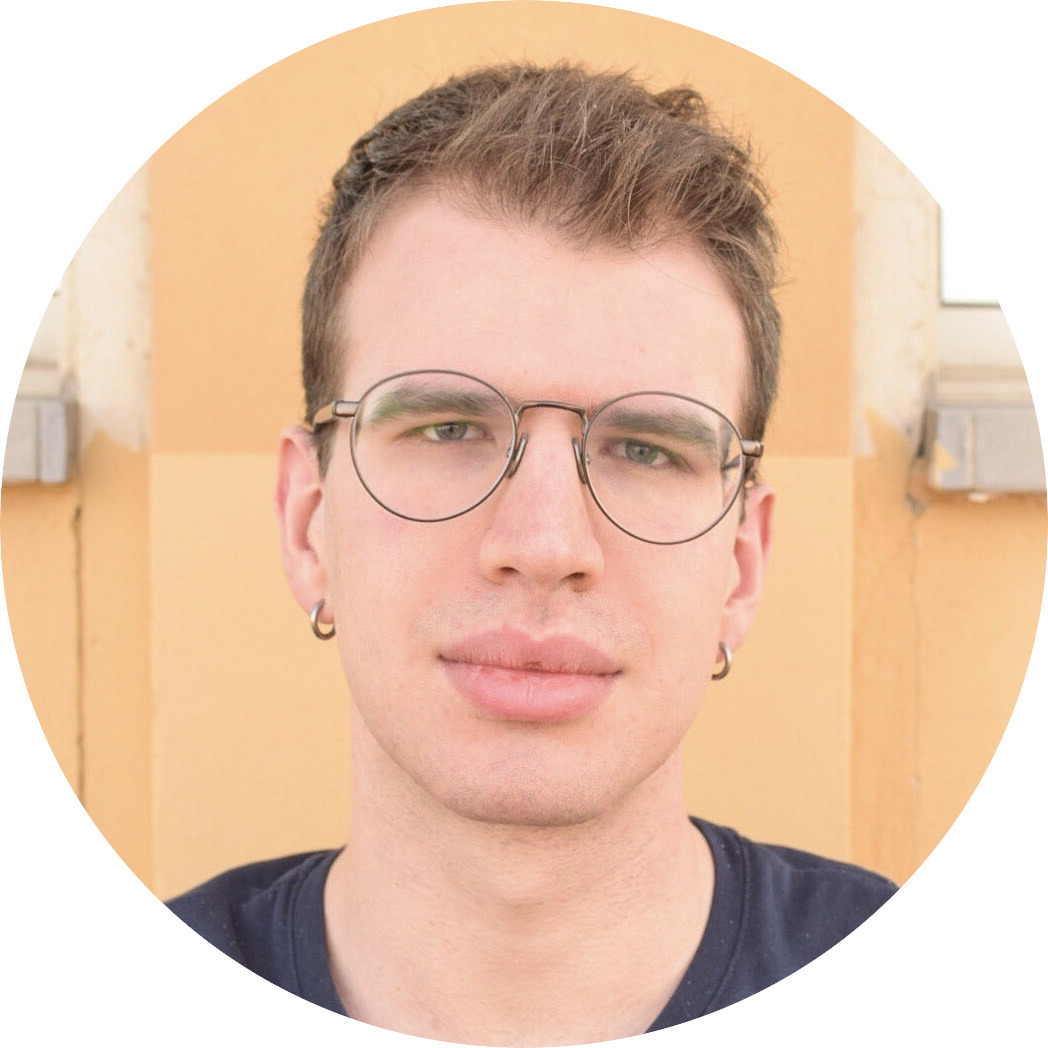
\includegraphics[width=3cm]{frickkm.JPG}}

}
\makeatother
% Headings spacing

\titlespacing\section{0pt}{2pt plus 2pt minus 2pt}{2pt plus 2pt minus 2pt}
\titlespacing\subsection{0pt}{2pt plus 2pt minus 2pt}{2pt plus 2pt minus 2pt}
% List spacing
\setlist{nosep, leftmargin=*}
\setlist{parsep=1pt, topsep=1pt, itemsep=1pt, leftmargin=*}
\title{Kevin Michael Frick}
\author{}

\begin{document}


\maketitle
\vspace{-0.8em}
\hrulefill


\section*{Education}

\textbf{MSc Computer Engineering} | University of Bologna | 09/2020 - Present | GPA: 29.8/30
\begin{itemize}
\item Student at the \emph{Collegio Superiore}, the \textbf{honors program} of the University of Bologna, offering additional \textbf{advanced and interdisciplinary education}.
Admission is solely based on \textbf{merit}.
Students are provided exemption from annual fees, free accommodation, an annual \textbf{scholarship} and the \textbf{tutorship} of a distinguished professor, in my case prof. Paolo Torroni, throughout their bachelor's and master's degrees.
Admission rate: <5\%.
\item \textbf{Student representative} to the Network of Italian Students in Schools and Institutes for Higher Study (RIASISSU) in 2020 and 2021.
Responsible for organizing and coordinating joint activities between Italian honors colleges.
\item Consolidated quantitative reasoning skills with courses in \textbf{operations research} and mathematical optimization, search-, learning-, and planning-based \textbf{artificial intelligence}, \textbf{game theory} and viability of \textbf{business projects}.
Attended additional courses about \textbf{mathematical methods} for artificial intelligence as well as equality and efficiency in \textbf{taxation policies} at Collegio Superiore.
\item Erasmus+ exchange at the Universitat Politècnica de Catalunya, Barcelona, for the entire second year, with a study plan focused on \textbf{machine learning}, mathematical \textbf{optimization} and algorithmic \textbf{game theory}.

\end{itemize}
\textbf{BSc Computer Engineering} | University of Bologna | 09/2017 - 07/2020 | Summa Cum Laude, GPA: 29.6/30
\begin{itemize}
\item Thesis: "Machine Learning for Semantic Visual SLAM", supervisors: prof. Stefano Mattoccia (University of Bologna) and prof. Stefano Stramigioli (University of Twente). Tutor at Collegio Superiore: prof. Elena Zattoni.
\item Strongly \textbf{quantitative} study plan, taking courses in advanced multivariate \textbf{calculus}, \textbf{numerical analysis}, C++11/14, Java, R, Go, Matlab and Python \textbf{programming}, \textbf{statistical modeling}, \textbf{economics and business organization}.
Attended additional courses in game theory, cryptocurrency and \textbf{blockchain design} and \textbf{optimal control} in economics at Collegio Superiore.
\end{itemize}

\section*{Work experience}
\textbf{Computer Vision Research Intern} | Robotics and Mechatronics, University of Twente, Netherlands | 03/2020 - 06/2020

\begin{itemize}
\item Erasmus+ traineeship with the goal of improving the \textbf{localization and mapping} (SLAM) capabilities of an unmanned aerial vehicle through \textbf{research and deployment} of deep \textbf{neural networks} for semantic segmentation of 3D scenes.
\item Developed a module for the ROS framework able to integrate a state-of-the-art SLAM solution with neural networks that make use of TensorFlow's, TensorFlow Lite's and PyTorch's \textbf{C++ and Python} APIs.
\item Developed and deployed a \textbf{Docker} container that significantly reduced environment set-up times and compatibility issues.
\end{itemize}

\section*{Languages}

\textbf{Italian}, native speaker | \textbf{English}, CEFR C2, IELTS Academic 8.5 | \textbf{Spanish}, CEFR B2 university certification

\section*{Projects, honors and awards}
\begin{itemize}
\item Selected to attend the \textbf{Cornell, Maryland, Max Planck Pre-doctoral Research School 2021}, a summer school aimed at \textbf{top students in computer science} interested in pursuing a PhD track.
The school included lectures on frontier research topics in computer science as well as panel discussions on how to plan and improve a career path in academic or private research.
\item As a student in Collegio Superiore, every year I write 5 papers based on \textbf{individual research} on topics addressed during the courses.
Selected titles include ``What can economsts learn from machine learning?'' (published 2020), ``Computer science and engineering tools for resource economics'', ``The platformization of the Internet infrastructure: economic and social effects in cities''.
\item Led a team of 4 people to develop an \textbf{artificial intelligence} able to play the Nordic board game Tablut using informed tree search techniques, training metaparameters with a genetic algorithm.
Project completed in spring 2021.
\item Developed a parallelized implementation of the \textbf{Q-learning} algorithm leveraging \textbf{Xilinx FPGA} hardware using high-level synthesis tools.
Project completed in spring 2021.
\item One of 6 students selected to compete in the national final of the the \textbf{CyberChallenge.IT}, specializing in software security, reverse engineering and system administration.
Attended the local training program in spring 2021, an advanced course in cryptography, malware analysis, software and web security.
Admission rate: <15\%.
\item Game engine pathfinder: developed a \textbf{pathfinding solution} in fall 2019 that is able to efficiently find optimal and collision-free paths for an arbitrary number of actors in an \textbf{open source game engine}.
Languages and libraries involved: C++11, Python 3, SDL, OpenAL
%\item Academic \textbf{software engineering} project, spring 2020: led a team of 3 people to detail an in-depth requirements, domain and risk analysis and develop a software solution to manage a bike rental service.
% Personally designed mock-ups of the UI using Figma.
% Languages and frameworks involved: Azure App Service, C\# 8.0, .NET Core 3.1, Azure SQL, Entity Framework Core, Bootstrap 4, jQuery.
% \item OrarioSync: \textbf{web application} that allows users to download their college timetables and allow for phone calendar synchronization. Languages and frameworks involved: Python 3, ZEIT Now v2, JavaScript ES6, React
\item Italian national selection for the International Olympiad in Informatics (IOI): \textbf{bronze medal} won in the 2016 final round of individual competitions, \textbf{third place} in the 2016 final round of team competitions.


\end{itemize}

\section*{Teaching activities}


\begin{itemize}
  \item Course in \textbf{Argumentation in Artificial Intelligence} \hfill Teaching Assistant to prof. Paolo Torroni | University of Bologna, fall 2021
  \item BSc course in \textbf{Software Engineering} \hfill Teaching Assistant to prof. Marco Patella |  University of Bologna, 2021
  \item High school course in \textbf{Competitive Programming} \hfill Teacher | Istituto Tecnico Aldini Valeriani, Bologna, 2020-2021
  \item High school course in \textbf{Computer Science} \hfill Teacher |  Istituto Tecnico Aldini Valeriani, Bologna, 2020-2021
\end{itemize}
\nocite{*}
\bibliography{CV}
\end{document}
